\section{The Muon System}
\label{sec:muon_sys}

Although it is the farthest system from the interaction point, the muon system is one of the most important within the Compact \emph{Muon} Solenoid detector.
%  is the {\bf Muon System} and is what puts the {\it Muon} in Compact {\it Muon} Solenoid.
Of the particles emerging from the interaction point, electrons and photons are absorbed by the ECAL (subsec.~\ref{subsec:ecal}), hadronic matter is absorbed by the HCAL (subsec.~\ref{subsec:hcal}), but muons are not stopped due to their relatively heavy mass (105.7 \MeV) for a lepton.
The only \emph{detectable} particles remaining at this point are muons, which interestingly will travel way outside of CMS before decaying, upwards of 100s of kilometers before decaying to an electron and neutrino (neutrinos are the only particles which CMS can't explicitly detect).
% We can only assume that we produced neutrinos when momentum is apparently not conserved in an event. 
% When the protons collide at the IP they have nearly zero momentum perpendicular to the beam pipe. 
% This is called transverse momentum, because it's well... transverse to the beam pipe, the z direction.
% If we track, tag, capture all the outgoing particles and reconstruct their transverse momenta, 
% if we find out that it is NOT zero by a large amount, then we say that 

The main purpose of the Muon System is to precisely determine the position and timing of muons.
% \begin{enumerate}
%     \item 
%     % for offline analysis.
%     \item Generate muon trigger primitives for the Level-1 trigger system.
% \end{enumerate}
Similar to the Silicon Tracker, the Muon System doesn't try to capture the muons passing through it;
instead it just tracks their positions. 
% In fact our very own Andrey, Guenakh, and Darin have been instrumental in implementing CSCs. 
% There's also an assembly hall downstairs where CSCs were constructed and tested 
% The  specializes muons. Au contraire; it \textit{specializes} in muon detection. 
% The Compact \textit{Muon} Solenoid would be a pretty hypocritical name if CMS did not detect muons. Au contraire; it \textit{specializes} in muon detection. 
% P
%It would be an ironic name if it did not detect muons well. 
The Muon System is comprised of three kinds of gaseous detectors: 
\begin{enumerate}
    \item {\bf Drift Tubes} (DTs) found in the barrel.
    \item {\bf Resistive Plate Chambers} (RPCs) found in both the barrel and endcap.
    \item {\bf Cathode Strip Chambers} (CSCs) found only in the endcap.
\end{enumerate}
Each of these technologies is constructed differently and was designed with a specific purpose. 
% In Chapter~\ref{ch:CSC}, the inner-workings of the CSCs are explained.

This concludes the overall design and purpose of the subdetectors that make up CMS.
Since I have had hands-on experience working on CSCs, I will discuss the CSC components and how it works in more detail in the subsection below.

\subsection{Let Me See These CSCs}

A cathode strip chambers (CSC) is a gaseous detector which specializes in muon detection. 
{\bf Quick Mention:} The University of Florida has been one of the main contributors to the CSC system and was home to one of the testing and assembly facilities before shipping the CSCs off to CERN.
The CSCs are found only on the endcaps of CMS and each endcap holds 270 CSCs (Fig~\ref{fig:cms_endcap}). 
%%%%%%%%%%%%%%%%%%%%
\begin{figure}[pbth]
\centering
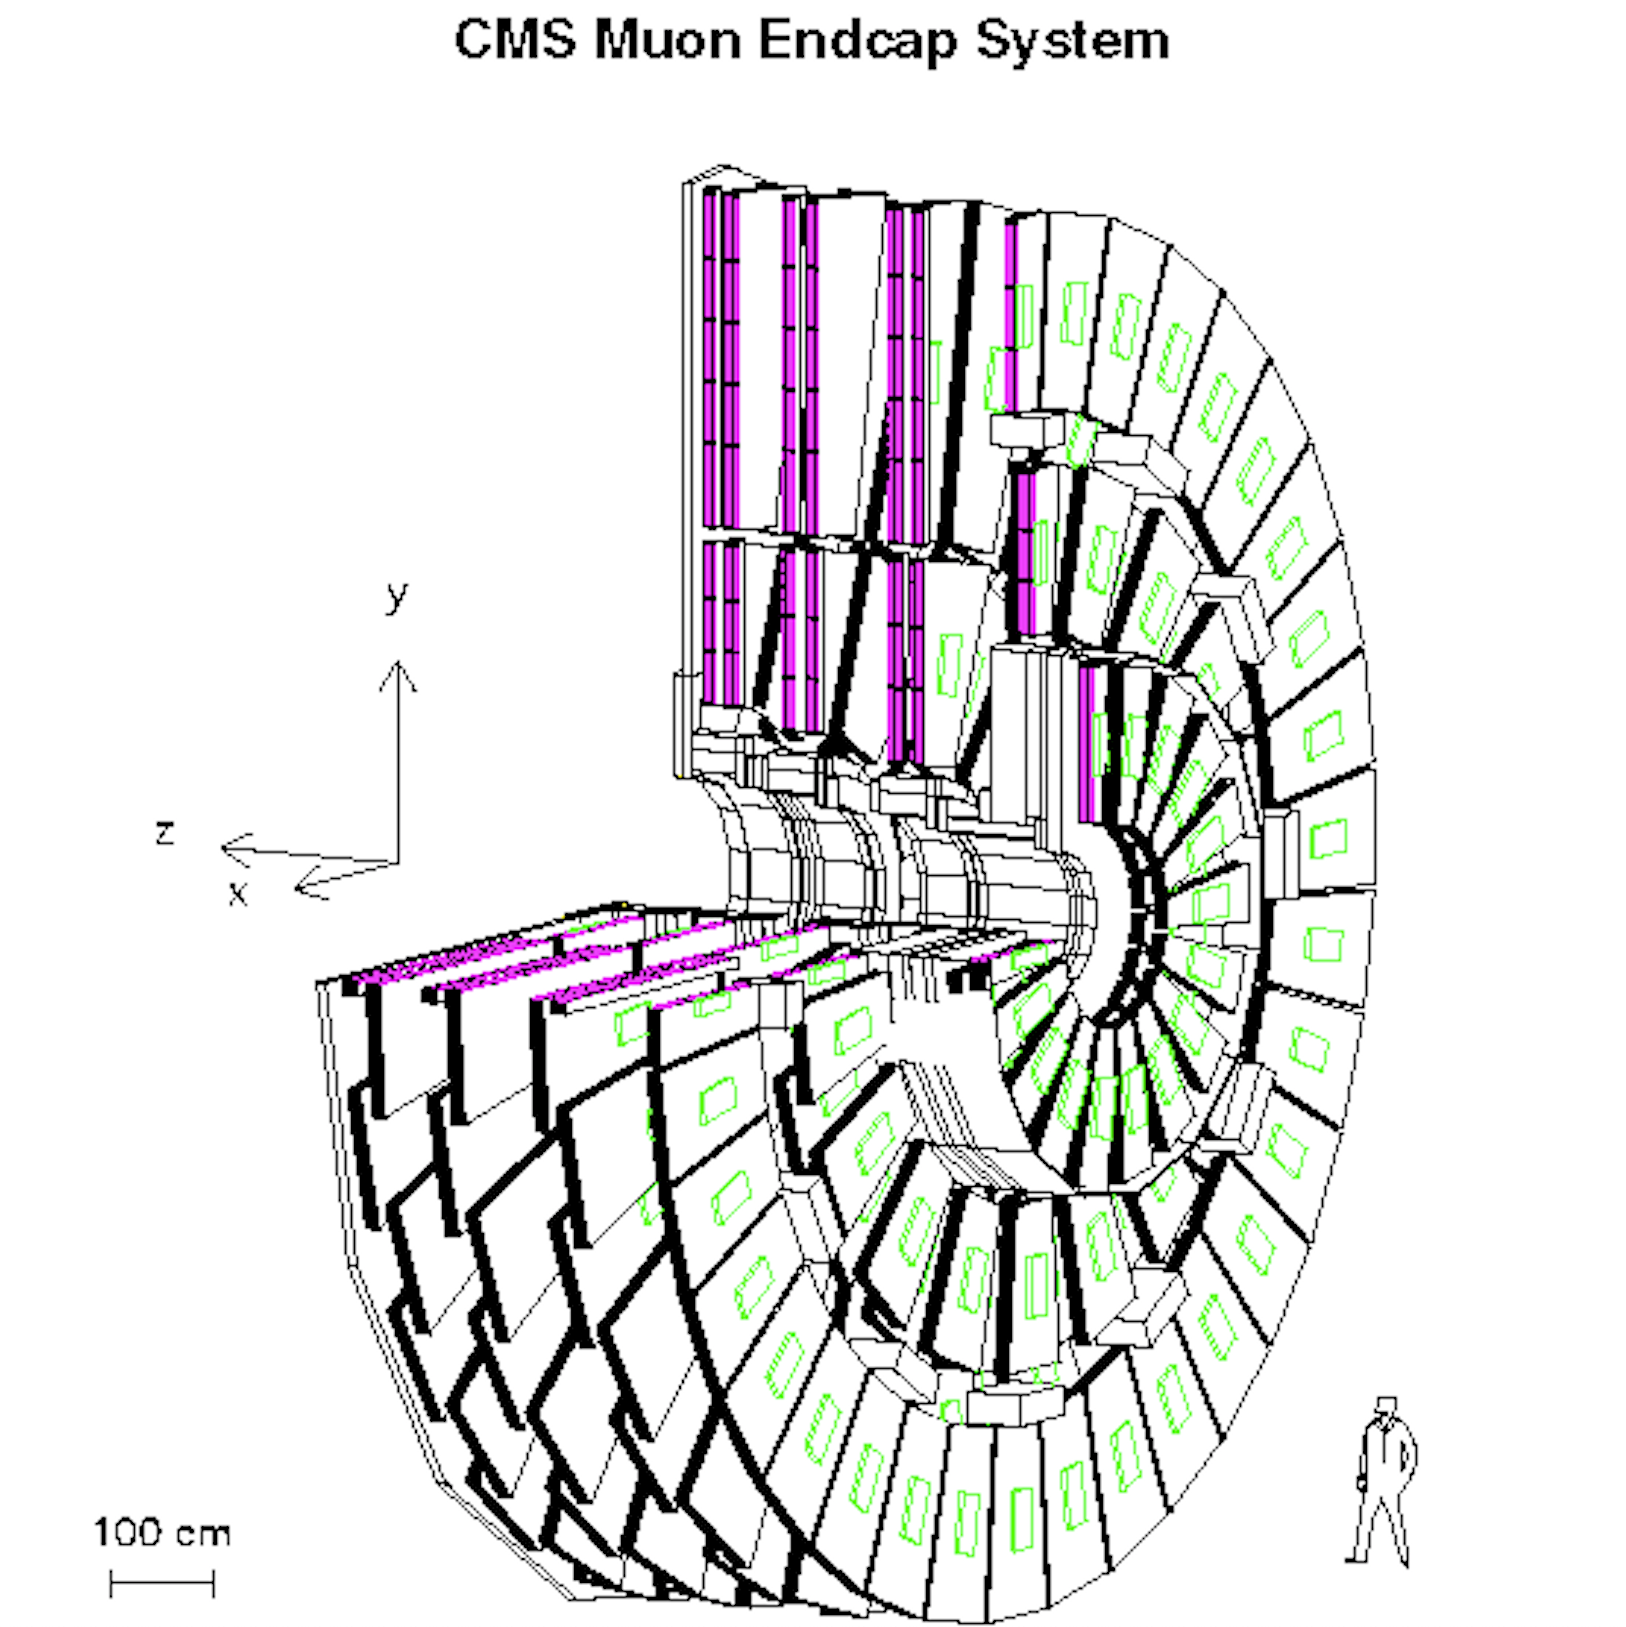
\includegraphics[width=0.49\textwidth,height=10cm,keepaspectratio]{figures/cms/muonsys/csc_endcap_cutaway.png}
\includegraphics[width=0.49\textwidth,height=10cm,keepaspectratio]{figures/cms/muonsys/csc_endcap_real.png}
    \caption{
    (Left) A cut out view of the ME+ endcap, simulated. Also shown is the coordinate system that CMS uses.
    (Right) The actual ME-2 disk is shown, revealing its ME-2/1 and ME-2/2 rings of CSCs.
    }
    \label{fig:cms_endcap}
\end{figure}
%%%%%%%%%%%%%%%%%%%%
Each CSC cost about \$100,000 to make, so very quickly this becomes an expensive project.
They are trapezoidal in shape and are composed of 6 layers filled with gas.
The gas surrounds wires and strips which are put under 3,600 V to aid in muon detection as explained below (Fig.~\ref{fig:csc_guts}). 
%%%%%%%%%%%%%%%%%%%%
\begin{figure}[pbth]
\centering
\includegraphics[width=0.49\textwidth,height=10cm,keepaspectratio]{figures/cms/muonsys/csc_cutaway_view_new.png}
\includegraphics[width=0.49\textwidth,height=10cm,keepaspectratio]{figures/cms/muonsys/csc_stripsandwires.png}
    \caption{
    (Left) A CSC with its top layer exposed. You can see very thin gold-plated tungsten wires which actually span the entire width of the CSC. 
    Thicker vertical strips run along the length.
    (Right) More detail showing the radial strips and the horizontal wires. Also shown is the 5 segments of a CSC.
    }
    \label{fig:csc_guts}
\end{figure}
%%%%%%%%%%%%%%%%%%%%
The gaseous mixture of $\mathrm{Ar:CO_{2}:CF_{4}}$ in the ratio of $5:4:1$ has been specially designed to maximize the lifetime of the CSC as it endures radiation damage over the years. 
In each layer, the gas mixture surrounds approximately 80 copper strips, each about 1 cm wide that span radially away from the IP.
Also inside the layers are over 1,000 gold-plated tungsten wires, which run azimuthally in the CMS coordinate system.
When the strips and wires detect muons they provide an (x,y) coordinate system to track the muon. 
As the muon passes through the remaining layers of the CSC, this provides a z coordinate as well, giving the Muon System the ability to ``see'' the full muon trajectory.
% In conjunction with the Silicon Tracker measurements, muon momentum can be measured to a precision of 

\textbf{Labelling the CSCs:} 
The two endcaps are labelled as ``ME+'' and ``ME-'', depending on in which z-direction they sit. 
Since they are structurally the same, let's focus on the ME+ endcap for a moment. 
The ME+ endcap has four disks, where ME+1 is the first disk, the one closest to the IP, and ME+4 is the fourth and farthest away. 
Similarly for the ME$-$ endcap. 
Then, within each disk, there are either two or three ``rings'' of CSCs, as shown in Fig~\ref{fig:cms_long_view_subdetectors} (green).
These rings are labelled like ME+2/1, which would indicate the second disk and the first (innermost) ring, radially closest to the IP.
All rings contain 36 CSCs, except for ME$\pm X$/1, for $X=$ 2,3,4, which contain only 18 CSCs.
Finally, the CSCs are given one, last number to label them on the ring:
the CSC that sits along the positive x-axis in CMS's coordinate system is given the number ``01'', \eg\ ME+4/2/01. 
The CSCs are then numbered incrementally following the positive azimuthal direction.
%%%%%%%%%%%%%%%%%%%%
\begin{figure}[pbth]
\centering
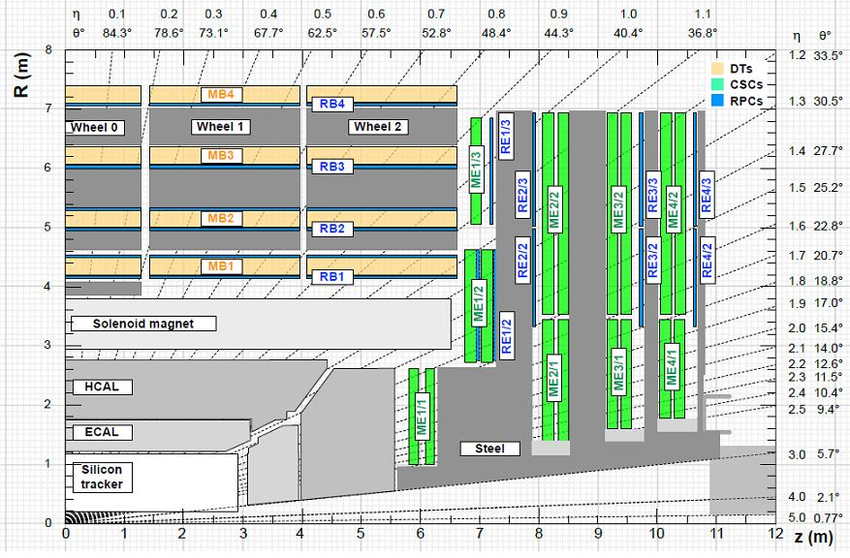
\includegraphics[width=15cm,height=10cm,keepaspectratio]{figures/cms/cms_longitudinal_view.png}
    \caption{
    Longitudinal cross section of CMS, showing the different pseudorapidity values ($\eta$) and also the different subdetector regions.
    }
    \label{fig:cms_long_view_subdetectors}
\end{figure}
%%%%%%%%%%%%%%%%%%%%

{\bf Detecting Muons:}
When a muon passes through a layer of a CSC, it has the chance to ionize an Ar atom (Fig.~\ref{fig:elec_avalanche}).
Since the wires are under high voltage (3,600 V), the ionized electron accelerates towards the positively-charged wire, and in doing so it ionizes many Ar atoms which are along its path. 
Starting from just a single electron, the multiplicity can go as high as 100,000 ionized electrons, thereby creating what is known as an electron avalanche. 
This phenomenon is called ``gas gain''.
%%%%%%%%%%%%%%%%%%%%
\begin{figure}[pbth]
\centering
\includegraphics[width=15cm,height=10cm,keepaspectratio]{figures/cms/muonsys/csc_elec_avalanche_old.png}
    \caption{
    A muon passes through one of the gaseous layers of the CSC, ionizing the gas mixture and inducing a charge on the wires and strips. 
    }
    \label{fig:elec_avalanche}
\end{figure}
%%%%%%%%%%%%%%%%%%%%
The electrons travel onto the wire and become an electrical signal which then gets sent to the anode front-end boards (AFEBs) for further signal processing.
The ionized Ar$^+$ will similarly distribute a charge signal on the negative strips. 
This cluster of charge is much more widely spread over the strips compared to the charge on the wires.
Therefore, comparator logic is implemented to narrow down the precision to the order of 100 $\mu$m by using half-strip information (Fig.~\ref{fig:comparators}).
%%%%%%%%%%%%%%%%%%%%
\begin{figure}[pbth]
\centering
\includegraphics[width=15cm,height=10cm,keepaspectratio]{figures/cms/muonsys/csc_comparators_and_strips.png}
    \caption{
    (Left) Comparators are used to compare neighboring strip cluster charge to determine on which half-strip the peak charge resided.
    (Right) A muon passes through all six layers of a CSC inducing charge on various half-strips.
    % cathode front-end board (CFEB) 
    }
    \label{fig:comparators}
\end{figure}
%%%%%%%%%%%%%%%%%%%%

The muon will continue passing through the next 5 layers, repeating the process of ionizing the gas mixture, and depositing an electrical signal on the wires. 
he wires and strips provide (x,y)-coordinates, and as the muon passes through the CSC, the other layers provide a z-coordinate, revealing the path of the muon.
% The AFEBs then digitize this analog signal using ADCs and 
Depending on how many hits were recorded by the CSC will determine if a muon event was significant enough to be registered as a real muon. 
If so, then its precise positions on the wires and strips will be read out by the Data Acquisition (DAQ) system and be stored for further data analysis.

% \subsection{Endcap Muon Electronics}
% In order to conclude that a muon definitely passed by the muon detectors, a very sophisticated electronics system has been developed. 

% Hmm... EMU is just for the endcaps. This system is called "EMU" and 

% I had been working on CMS analyses for about a year and a half before I actually saw CMS just earlier this year. And let me tell you: It is HUGE! 
% Next I am going to elaborate more on the CSCs, since my first experience with CMS hands-on work with CSCs. 

% The muon barrel system, after it talks with the tracker system, has a muon pT resolution of 1.5% in the barrel and ~6% in the endcap.

% Trigger system:
% Since the event  rate and data rate are so high, and most of the events are uninteresting, typical physics,
% we need a fast-working filtration system to sift through the good and bad events. 
% We want to "trigger" on the good events but only have about 4 μs to do so. 
% This is the job of the L1 trigger and and the High-Level Trigger. 
% I'm not going to explain any more of this because it is an extremely sophisticated system. 

\subsection{Drift Tube Chambers}
\label{subsec:drifttube}

\subsection{Cathode Strip Chambers}
\label{subsec:csc}

\subsection{Resistive Plate Chambers}
\label{subsec:rpc}